\documentclass[11pt,a4paper]{article}
\usepackage[utf8]{inputenc}
\usepackage[T1]{fontenc}
\usepackage{lmodern}
\usepackage{microtype}
\usepackage{graphicx}
\usepackage{xcolor}
\usepackage{geometry}
\usepackage{hyperref}
\usepackage{listings}
\usepackage{booktabs}
\usepackage{amsmath}
\usepackage{tikz}
\usepackage{fancyhdr}
\usepackage{tcolorbox}
\usepackage{enumitem}

% Page geometry
\geometry{margin=2.5cm}

% Define colors
\definecolor{cvutblue}{RGB}{0, 83, 155}
\definecolor{lightgray}{RGB}{240, 240, 240}
\definecolor{darkgray}{RGB}{64, 64, 64}
\definecolor{commentgreen}{RGB}{0, 130, 0}

% Set up hyperref
\hypersetup{
    colorlinks=true,
    linkcolor=cvutblue,
    filecolor=cvutblue,
    urlcolor=cvutblue,
    citecolor=cvutblue,
    pdftitle={NB-IoT Camera Documentation},
    pdfauthor={Pavel Travnicek},
}

% Set up code listings
\lstset{
    basicstyle=\ttfamily\small,
    keywordstyle=\color{blue}\bfseries,
    commentstyle=\color{commentgreen},
    stringstyle=\color{red},
    numbers=left,
    numberstyle=\tiny\color{darkgray},
    stepnumber=1,
    numbersep=8pt,
    backgroundcolor=\color{lightgray},
    showspaces=false,
    showstringspaces=false,
    showtabs=false,
    frame=single,
    tabsize=2,
    captionpos=b,
    breaklines=true,
    breakatwhitespace=false,
    escapeinside={\%*}{*)},
    morekeywords={*,define,do,done,elif,else,esac,fi,for,function,if,in,select,then,until,while}
}

% Header and footer
\pagestyle{fancy}
\fancyhf{}
\fancyhead[L]{NB-IoT Camera Documentation}
\fancyhead[R]{\today}
\fancyfoot[C]{\thepage}
\renewcommand{\headrulewidth}{0.4pt}
\renewcommand{\footrulewidth}{0.4pt}

% Define a nice box for highlights
\newtcolorbox{infobox}[1][]{
    colback=lightgray!30,
    colframe=cvutblue,
    fonttitle=\bfseries,
    #1
}

\begin{document}

% Title page
\begin{titlepage}
    \centering
    \vspace*{1cm}
    \vspace{1.5cm}
    {\Huge\bfseries ESP32 GPS Photo Uploader\par}
    \vspace{1cm}
    {\Large NB-IoT Camera System with GNSS, Deep Sleep, and Power Management\par}
    \vspace{1.5cm}
    {\Large\itshape Department of Physics\par}
    {\Large Czech Technical University in Prague\par}
    \vfill
    {\large \today\par}
\end{titlepage}

\tableofcontents
\newpage

\section{Introduction}

This document describes an ESP32-based IoT camera system that leverages NB-IoT technology for wireless communication, incorporating GNSS (Global Navigation Satellite System) for precise positioning, a high-quality camera for image capture, and comprehensive power management. The device is designed with power efficiency as its primary concern, employing various deep sleep strategies and intelligent power management techniques.

The system captures photos using an OV2640 camera module and transmits them over TCP connections, while simultaneously sending sensor data and GPS coordinates via UDP in Telegraf line protocol format. The device includes temperature and humidity monitoring, battery level tracking, and an OLED display for status information.

\begin{infobox}[title=Key Features]
\begin{itemize}[leftmargin=*]
    \item \textbf{NB-IoT Communication}: Cellular connectivity for reliable data transmission
    \item \textbf{High-Quality Camera}: OV2640 camera with configurable resolution and quality
    \item \textbf{GNSS Positioning}: Accurate location tracking with GPS/GLONASS support
    \item \textbf{Advanced Power Management}: Deep sleep modes and power cycling
    \item \textbf{OLED Display}: Visual status information and debugging
    \item \textbf{Environmental Monitoring}: Temperature and humidity sensing
    \item \textbf{Battery Monitoring}: Real-time battery status reporting
    \item \textbf{Dual Protocol Support}: TCP for photos, UDP for sensor data
    \item \textbf{Night Mode}: Extended sleep during night hours
    \item \textbf{DNS-Based Configuration}: Flexible server addressing
\end{itemize}
\end{infobox}

The device is particularly suited for applications requiring periodic photo capture and transmission with minimal power consumption, such as environmental monitoring, security surveillance, and smart city infrastructure. Its ability to operate on battery power for extended periods makes it ideal for deployment in remote or hard-to-access locations.

\section{Hardware Components}

The camera system integrates several hardware components, each serving a specific function in the overall system:

\begin{table}[h]
\centering
\begin{tabular}{@{}llp{8cm}@{}}
\toprule
\textbf{Component} & \textbf{Model} & \textbf{Function} \\
\midrule
Microcontroller & ESP32-S3 & Main processing unit with integrated Wi-Fi and Bluetooth (disabled for power saving) \\
Camera Module & OV2640 & High-quality image capture with configurable resolution \\
GNSS Module & DFRobot GNSS & Provides precise geographical coordinates \\
NB-IoT Modem & Quectel BC95 & Enables cellular connectivity for data transmission \\
Power Management & AXP313A & Manages camera power, battery monitoring, and power optimization \\
OLED Display & LD7032 60x32 & Shows device status and debug information \\
Environmental Sensor & AHT20 & Monitors temperature and humidity \\
Battery & Li-ion/LiPo & Power source with voltage divider monitoring \\
\bottomrule
\end{tabular}
\caption{Hardware components of the NB-IoT camera system}
\label{tab:components}
\end{table}

The following figures show the main schematic sections of the NB-IoT camera system:

\begin{itemize}
    \item FireBeetle 2 Board ESP32-S3 microcontroller and connectors
    \item NB-IoT BC95-G modem and supporting circuitry
    \item Solar charging and power management
\end{itemize}

\begin{figure}[h]
    \centering
    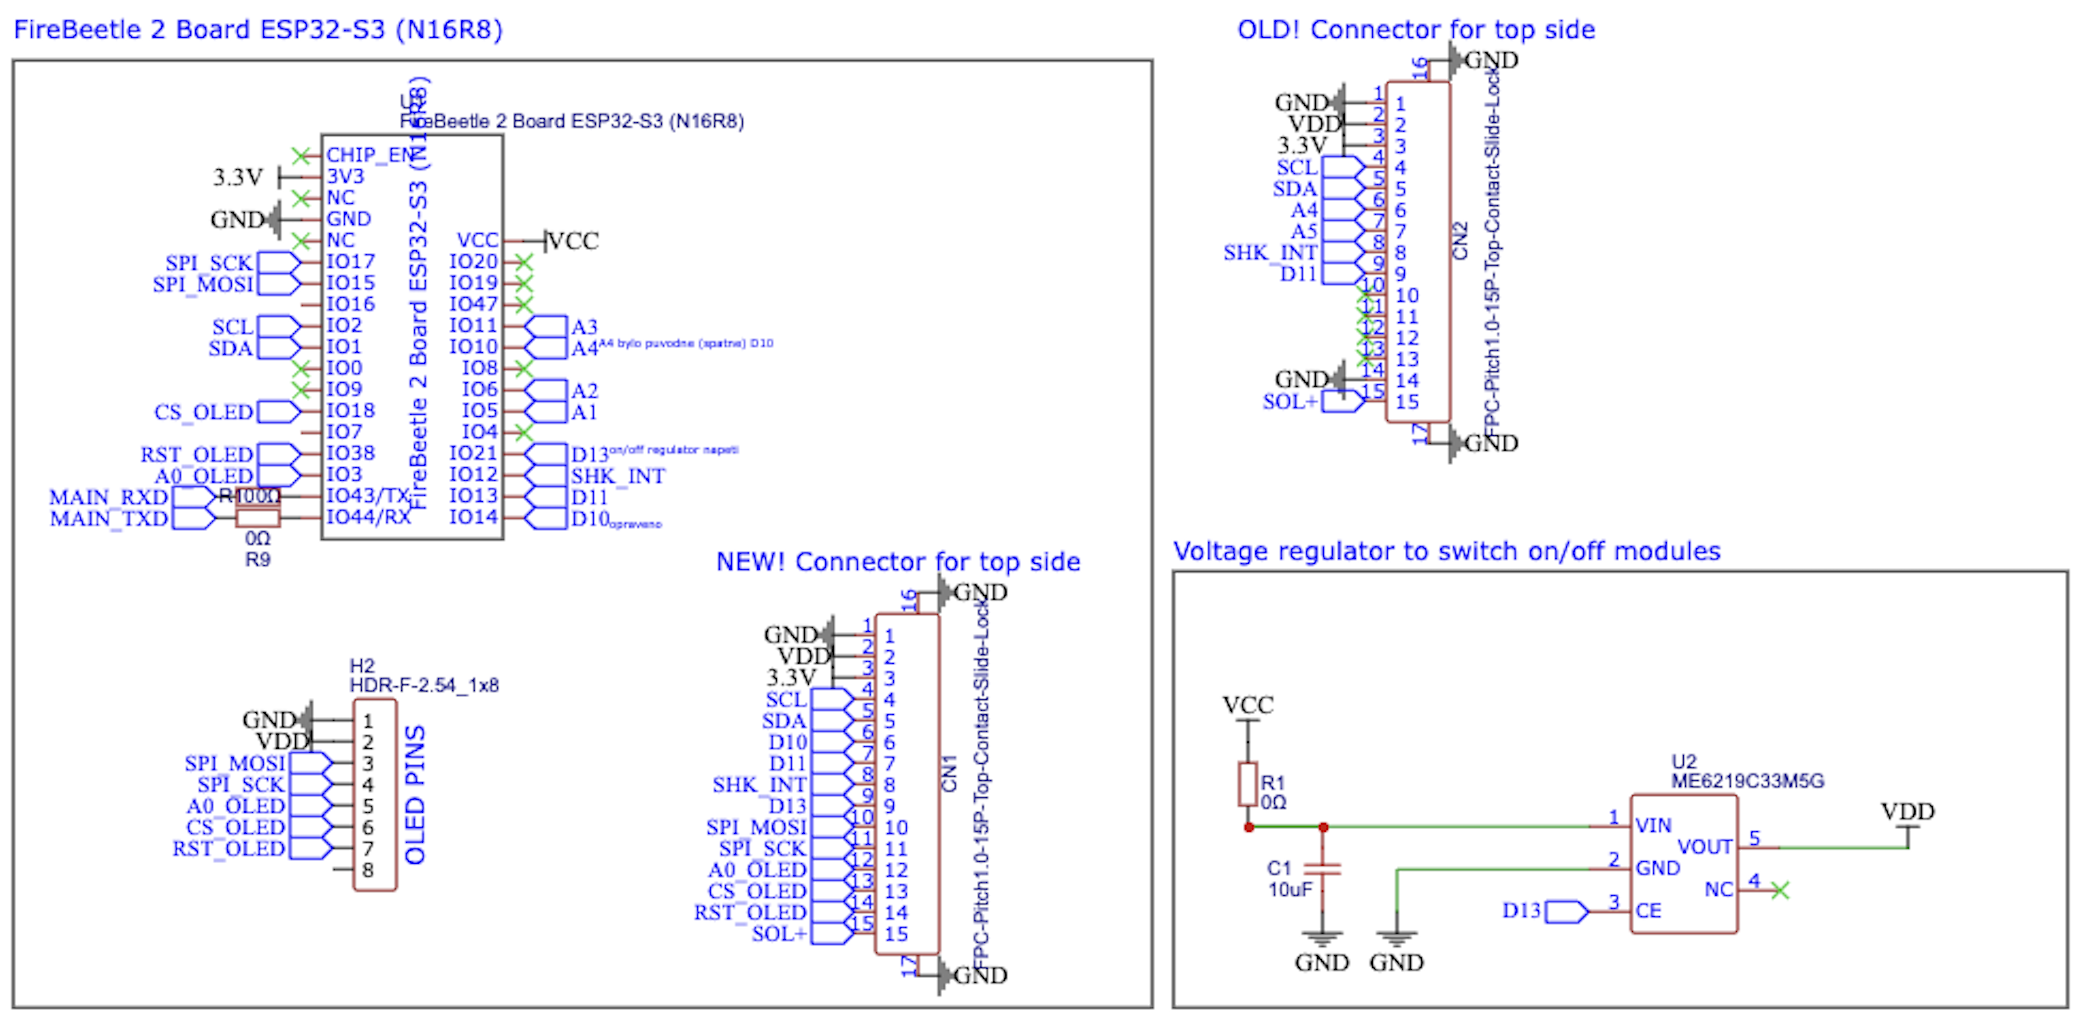
\includegraphics[width=0.95\textwidth]{tex_photos/schematic_firebeetle.png}
    \caption{Schematic: FireBeetle 2 Board ESP32-S3 microcontroller and connectors.}
    \label{fig:schematic-firebeetle}
\end{figure}

\begin{figure}[h]
    \centering
    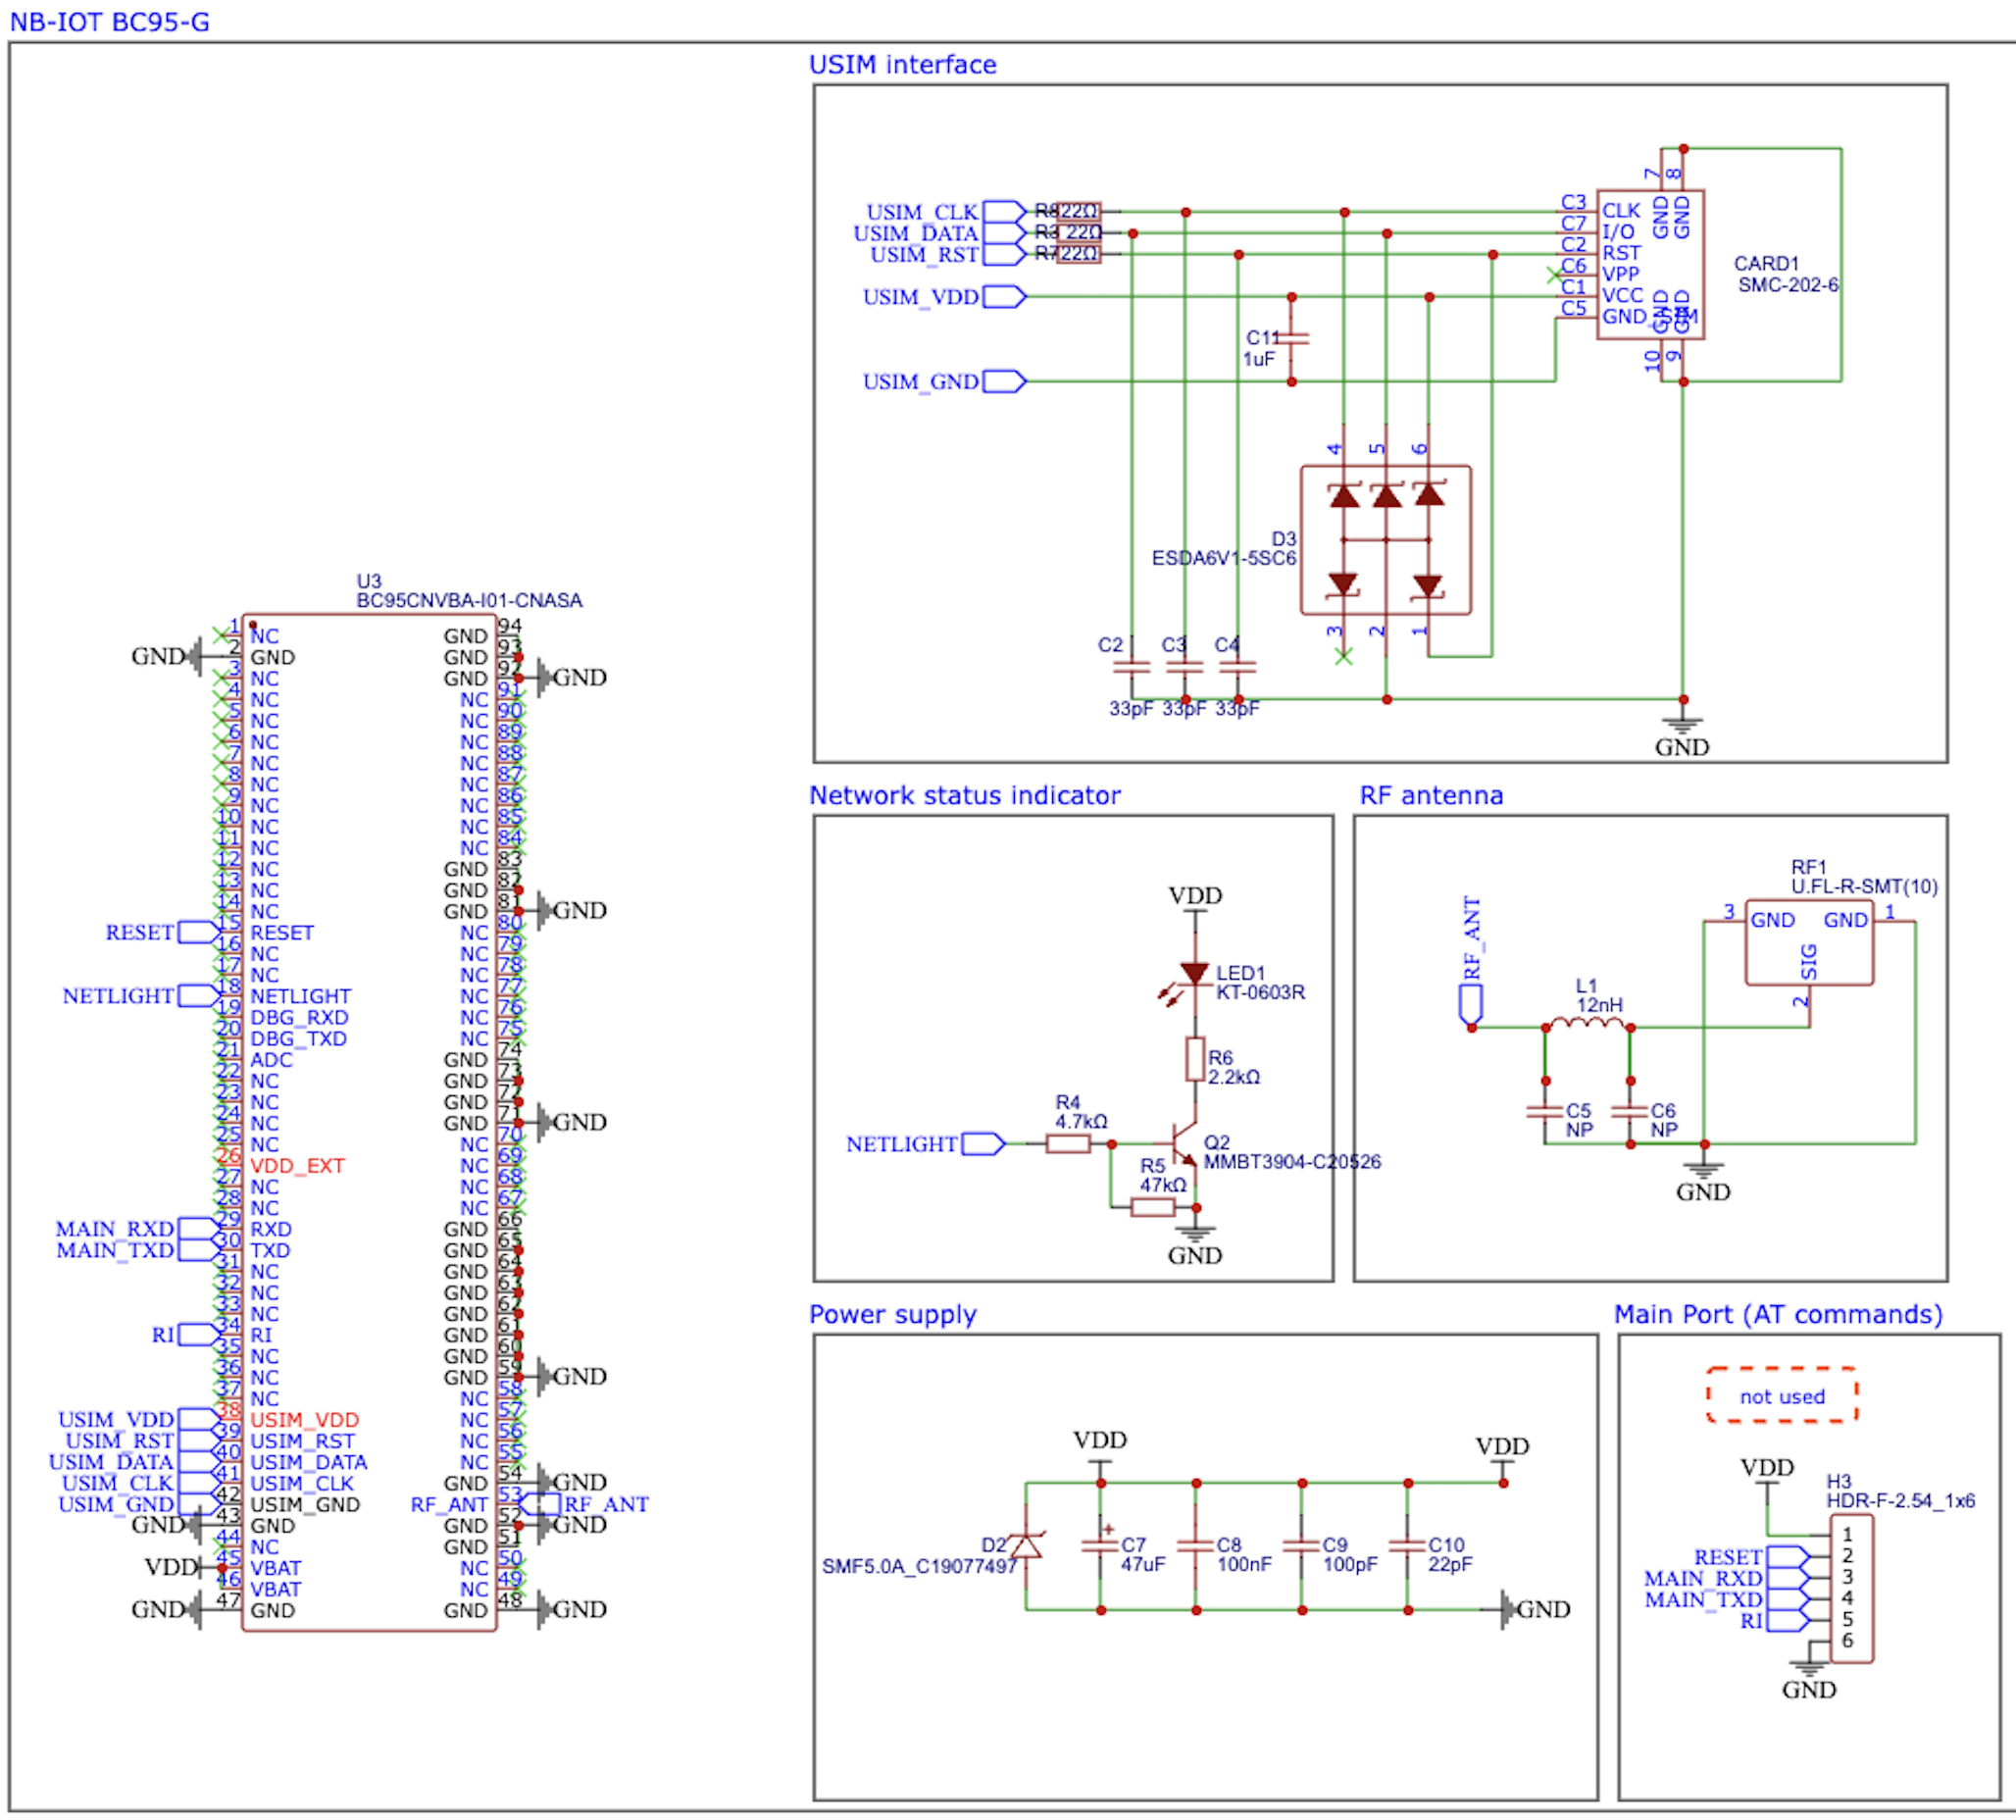
\includegraphics[width=0.95\textwidth]{tex_photos/schematic_nbiot.png}
    \caption{Schematic: NB-IoT BC95-G modem and supporting circuitry.}
    \label{fig:schematic-nbiot}
\end{figure}

\begin{figure}[h]
    \centering
    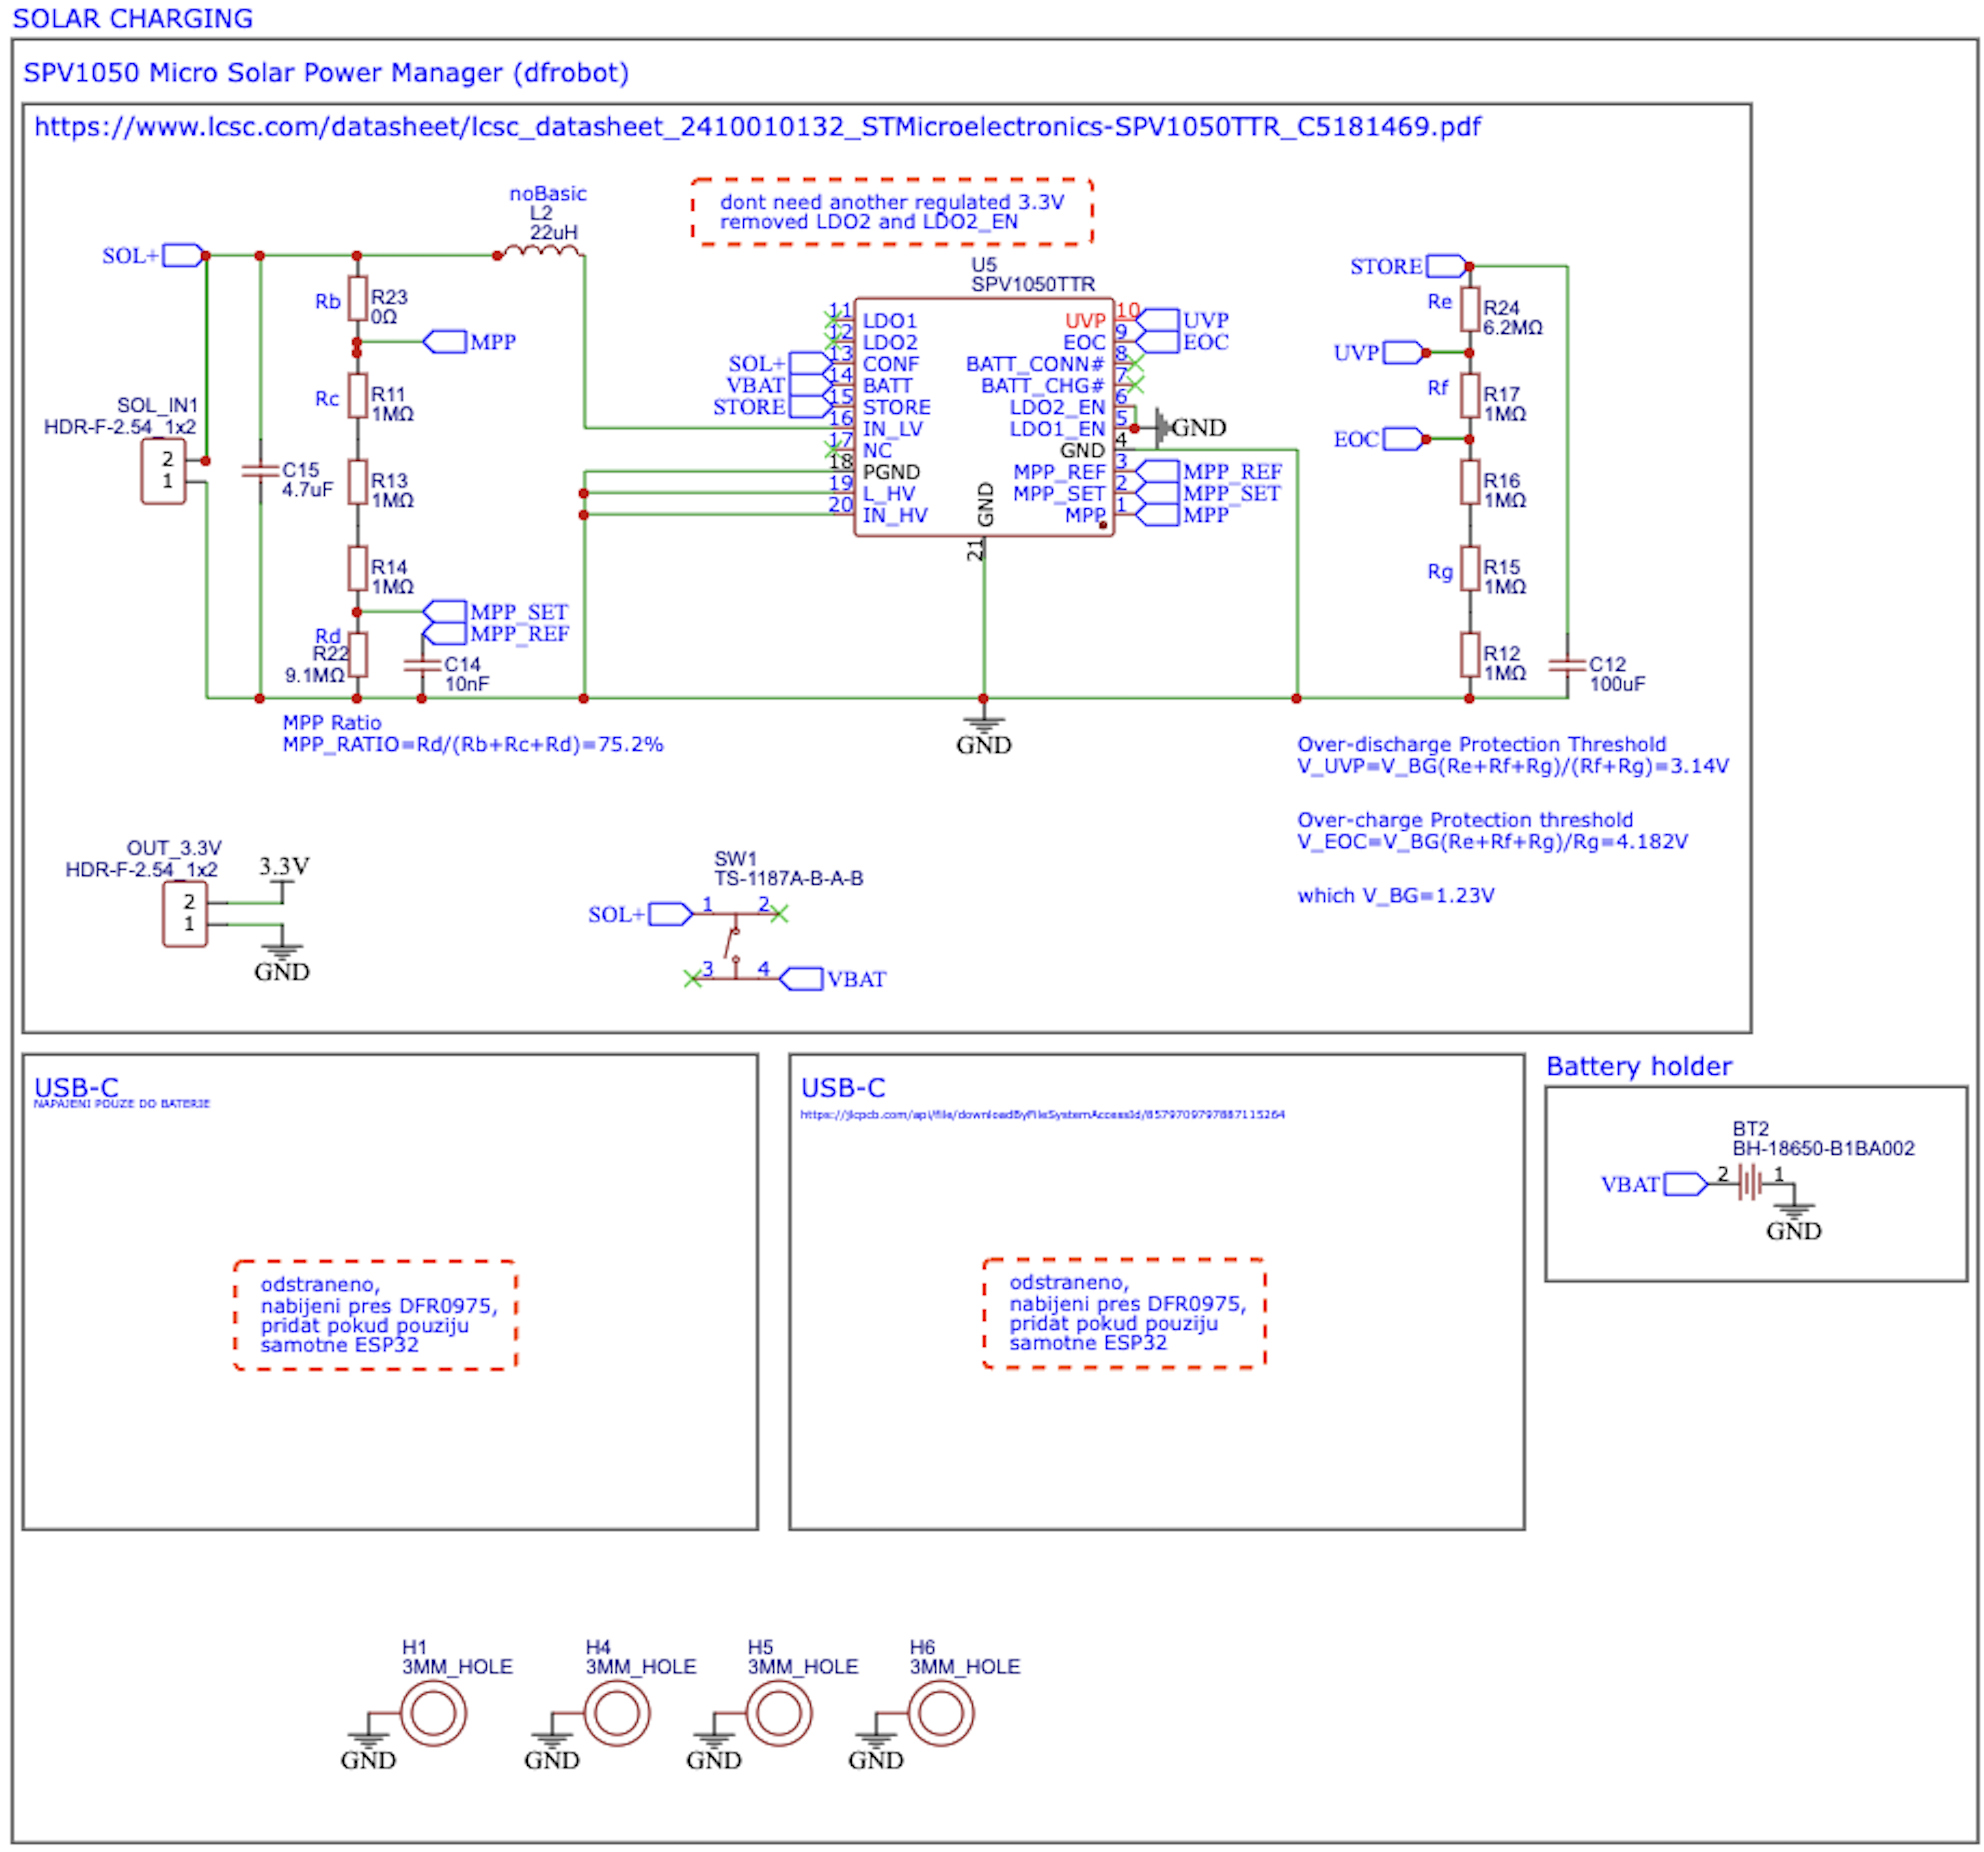
\includegraphics[width=0.95\textwidth]{tex_photos/schematic_solarcharging.png}
    \caption{Schematic: Solar charging and power management section.}
    \label{fig:schematic-solarcharging}
\end{figure}

% After the hardware table
\begin{figure}[h]
\centering
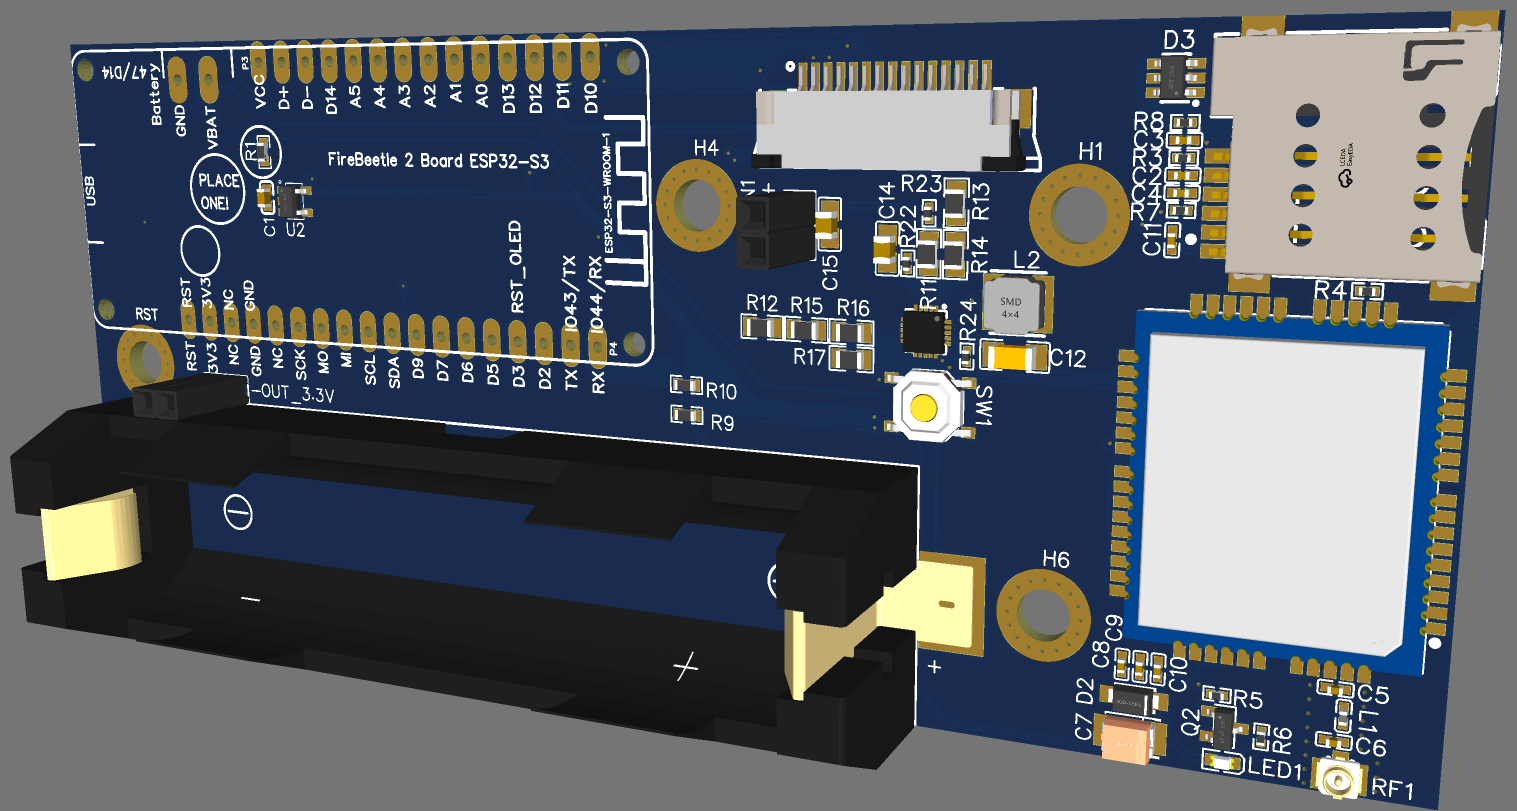
\includegraphics[width=0.85\textwidth]{tex_photos/nbiotcam_board.png}
\caption{3D model of the main NB-IoT camera PCB board.}
\label{fig:nbiotcam-board}
\end{figure}

% Add photo of the NB-IoT unit in the demolition container
\begin{figure}[h]
\centering
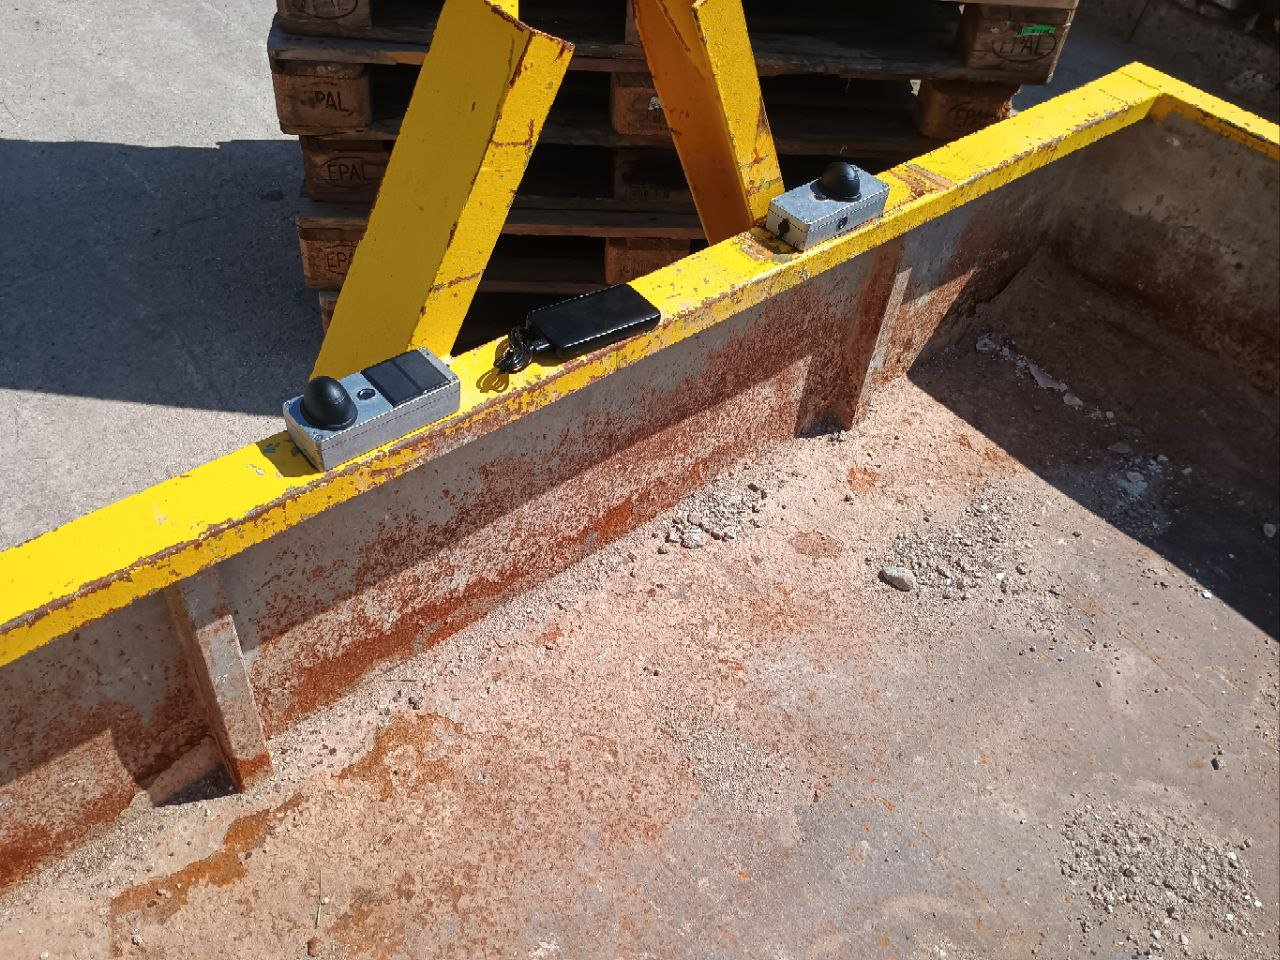
\includegraphics[width=0.85\textwidth]{tex_photos/5956168425011267555.jpg}
\caption{NB-IoT unit on the right, placed in a demolition container.}
\label{fig:nbiot-container}
\end{figure}

\subsection{ESP32-S3 Microcontroller}

The ESP32-S3 is a powerful, dual-core microcontroller with integrated Wi-Fi and Bluetooth capabilities. For this application, we specifically use features including:

\begin{itemize}
    \item Low deep-sleep current consumption
    \item Multiple sleep modes (light sleep, deep sleep, and hibernation)
    \item Programmable I/O pins with wake-up capability
    \item PSRAM support for high-quality image processing
    \item Hardware acceleration for cryptographic operations
\end{itemize}

\subsection{OV2640 Camera Module}

The OV2640 camera module provides high-quality image capture capabilities:

\begin{itemize}
    \item Resolution up to 1600x1200 pixels
    \item Configurable JPEG quality settings
    \item Automatic exposure and white balance control
    \item SCCB (I2C) interface for configuration
    \item 8-bit parallel data interface
\end{itemize}

\subsection{NB-IoT Communication}

The device uses a Quectel BC95 NB-IoT modem to communicate over cellular networks. NB-IoT offers several advantages for IoT applications:

\begin{itemize}
    \item Wide coverage area with cellular infrastructure
    \item Low power consumption compared to traditional cellular
    \item Reliable connectivity in challenging environments
    \item Support for both TCP and UDP protocols
    \item Cost-effective data transmission
\end{itemize}

\subsection{GNSS Module}

The GNSS module provides precise geographical positioning by receiving signals from multiple satellite constellations (GPS, GLONASS). Key features include:

\begin{itemize}
    \item Support for multiple satellite systems
    \item Configurable power modes
    \item I2C interface for communication with the ESP32
    \item Position accuracy to within a few meters
    \item Speed and course over ground information
\end{itemize}

\subsection{Power Management System}

The AXP313A power management IC provides comprehensive power control:

\begin{itemize}
    \item \textbf{Camera Power Control}: Dedicated power rail for the camera module
    \item \textbf{Battery Monitoring}: Real-time voltage and percentage monitoring
    \item \textbf{Power Optimization}: Automatic power cycling and sleep management
    \item \textbf{Voltage Regulation}: Multiple regulated outputs for different components
\end{itemize}

\section{Software Architecture}

The firmware is structured around power-efficient operation cycles, with careful management of active and sleep states. The main operational cycle consists of:

\begin{enumerate}
    \item Wake up (from timer or external interrupt)
    \item Initialize sensors and modules
    \item Acquire GNSS data (if enabled)
    \item Capture photo (if enabled)
    \item Transmit data via NB-IoT
    \item Enter deep sleep mode
\end{enumerate}

\subsection{Operational Modes}

The device supports configurable operational modes:

\begin{description}
    \item[Camera Mode] Captures and transmits photos over TCP with start/end markers
    \item[Sensor Mode] Transmits environmental and GPS data over UDP
    \item[Combined Mode] Both photo capture and sensor data transmission
    \item[Night Mode] Extended sleep periods during night hours
\end{description}

\subsection{Sleep Management}

Power efficiency is achieved through sophisticated sleep management:

\begin{itemize}
    \item \textbf{Deep Sleep}: The ESP32 and peripheral components are powered down between transmissions
    \item \textbf{Adaptive Sleep Duration}: Sleep times can be adjusted based on time of day
    \item \textbf{RTC Memory}: Critical state information is preserved in RTC memory
    \item \textbf{Wake-up Sources}: The device can wake from timer expiration
    \item \textbf{Component Power Cycling}: Individual components are powered down when not in use
\end{itemize}

\begin{figure}[h]
\centering
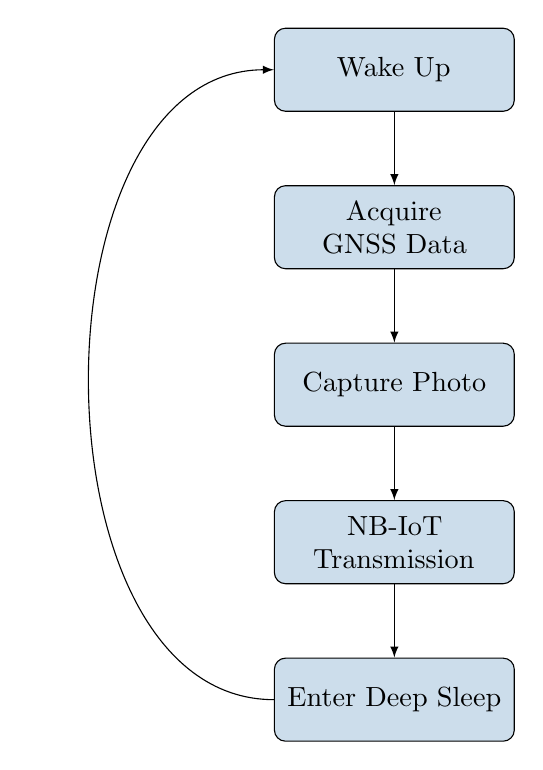
\begin{tikzpicture}[node distance=2cm, auto]
    % Define styles
    \tikzstyle{block} = [rectangle, draw, fill=cvutblue!20, text width=8em, text centered, rounded corners, minimum height=3em]
    \tikzstyle{line} = [draw, -latex]
    
    % Nodes
    \node [block] (init) {Wake Up};
    \node [block, below of=init] (gnss) {Acquire GNSS Data};
    \node [block, below of=gnss] (camera) {Capture Photo};
    \node [block, below of=camera] (transmit) {NB-IoT Transmission};
    \node [block, below of=transmit] (sleep) {Enter Deep Sleep};
    
    % Connections
    \path [line] (init) -- (gnss);
    \path [line] (gnss) -- (camera);
    \path [line] (camera) -- (transmit);
    \path [line] (transmit) -- (sleep);
    \path [line] (sleep) to [bend left=90] (init);
\end{tikzpicture}
\caption{Operational cycle of the NB-IoT camera system}
\label{fig:cycle}
\end{figure}

\section{Data Communication}

\subsection{NB-IoT Integration}

The device uses AT commands to communicate with the Quectel BC95 modem:

\begin{enumerate}
    \item Initialize the modem with proper configuration
    \item Register on the NB-IoT network
    \item Establish TCP/UDP connections as needed
    \item Transmit data with retry mechanisms
    \item Close connections and enter sleep mode
\end{enumerate}

\subsection{TCP Photo Transmission}

Photos are transmitted over TCP with special markers for reliable delivery:

\begin{table}[h]
\centering
\begin{tabular}{@{}ccl@{}}
\toprule
\textbf{Component} & \textbf{Size} & \textbf{Description} \\
\midrule
Start Marker & 4 bytes & [0x00, 0x00, 0x00, 0x00] \\
Photo Data & Variable & JPEG image data in chunks \\
End Marker & 4 bytes & [0xFF, 0xFF, 0xFF, 0xFF] \\
\bottomrule
\end{tabular}
\caption{TCP photo transmission format}
\label{tab:tcp}
\end{table}

\subsection{UDP Sensor Data Format}

Sensor and GPS data is transmitted in Telegraf line protocol format:

\begin{lstlisting}[language=text, caption=UDP Data Format]
gps_data,device=esp32 gpsFIX=true,temperature=23.1,humidity=45.2,battery=42
\end{lstlisting}

The data includes:
\begin{itemize}
    \item GPS fix status (true/false)
    \item Temperature in degrees Celsius
    \item Humidity percentage
    \item Battery percentage
\end{itemize}

\section{Power Optimization}

Several techniques are employed to minimize power consumption:

\subsection{Hardware Power Management}

\begin{itemize}
    \item \textbf{Power Gating}: The camera and GNSS modules are completely powered down when not in use
    \item \textbf{Modem Sleep}: The NB-IoT modem enters sleep mode between transmissions
    \item \textbf{WiFi/Bluetooth Disable}: These radios are disabled as they're not needed
    \item \textbf{Voltage Regulation}: Efficient power conversion and distribution
\end{itemize}

\subsection{Software Power Management}

\begin{itemize}
    \item \textbf{Adaptive GNSS Timeout}: The device limits how long it will wait for a GNSS fix
    \item \textbf{Modem Sleep}: The ESP32 is configured to enter modem sleep to reduce power
    \item \textbf{Night-time Scheduling}: Longer sleep periods are used during night hours
    \item \textbf{Component Initialization}: Only initialize components when needed
\end{itemize}

\subsection{Measured Power Consumption}

The device's power consumption varies significantly across different operational phases:

\begin{table}[h]
\centering
\begin{tabular}{@{}lccc@{}}
\toprule
\textbf{Mode} & \textbf{Current} & \textbf{Duration} & \textbf{Energy per Cycle} \\
\midrule
Deep Sleep & 15 µA & 3600 s & 54 mC \\
GNSS Acquisition & 70 mA & 10-120 s & 700-8400 mC \\
Camera Capture & 150 mA & 5-10 s & 750-1500 mC \\
NB-IoT TX & 200 mA & 2-5 s & 400-1000 mC \\
Processing & 50 mA & 3 s & 150 mC \\
\bottomrule
\end{tabular}
\caption{Power consumption in different operational states}
\label{tab:power}
\end{table}

\section{Data Integration}

The device integrates with backend systems through multiple pathways:

\subsection{NB-IoT Network}

Data transmitted by the device is first received by NB-IoT base stations and forwarded to the cellular network infrastructure, which then routes the data to the configured server.

\subsection{Node-RED Integration}

The device's data is processed using Node-RED flows that:

\begin{enumerate}
    \item Decode the TCP photo data and reconstruct complete images
    \item Parse UDP sensor data in Telegraf line protocol format
    \item Extract relevant fields (GPS coordinates, sensor readings, battery status)
    \item Forward data to storage or visualization systems
\end{enumerate}

\subsection{Server Configuration}

The device connects to a server at \texttt{www.iot-magic.com} using:

\begin{itemize}
    \item \textbf{TCP Port 8009}: For photo transmission
    \item \textbf{UDP Port 8094}: For sensor data
    \item \textbf{DNS Resolution}: Flexible server addressing without hardcoded IPs
\end{itemize}

\section{Setup and Configuration}

\subsection{Hardware Setup}

To configure the hardware:

\begin{enumerate}
    \item Connect the OV2640 camera to the designated GPIO pins
    \item Connect the GNSS module to the correct I2C pins
    \item Connect the BC95 modem using UART2 (pins 43/44)
    \item Connect the AHT20 sensor to I2C
    \item Connect the OLED display to the designated SDA/SCL pins
    \item Connect the AXP313A power management IC
    \item Connect the battery with voltage divider for monitoring
\end{enumerate}

\subsection{NB-IoT Configuration}

The device requires proper NB-IoT network configuration:

\begin{lstlisting}[language=C++, caption=NB-IoT Configuration]
// Server configuration
const String SERVER_IP = "www.iot-magic.com";
const int TCP_PORT = 8009;
const int UDP_PORT = 8094;

// Modem configuration
#define BC95_RX_PIN 44
#define BC95_TX_PIN 43
\end{lstlisting}

\subsection{Firmware Configuration}

Key firmware parameters that can be adjusted:

\begin{itemize}
    \item \textbf{Sleep Duration}: The default sleep time between transmissions (3600 seconds)
    \item \textbf{Camera Quality}: JPEG quality and resolution settings
    \item \textbf{GNSS Timeout}: How long to attempt to acquire a GNSS fix (120 seconds)
    \item \textbf{Night-time Parameters}: Configure different behavior during night hours
    \item \textbf{Retry Mechanisms}: Number of retry attempts for failed transmissions
\end{itemize}

\section{Applications and Use Cases}

The NB-IoT camera system is versatile and can be applied to various domains:

\subsection{Environmental Monitoring}

Capture images of environmental conditions while collecting sensor data for comprehensive monitoring of remote locations.

\subsection{Security and Surveillance}

Deploy units in areas requiring periodic visual monitoring with minimal power requirements and cellular connectivity.

\subsection{Smart City Infrastructure}

Monitor fixed infrastructure assets while providing visual context and location information.

\subsection{Research and Education}

The device serves as an excellent platform for academic research and educational purposes, demonstrating IoT principles, power optimization techniques, and image processing.

\section{Future Development}

Several enhancements are planned or possible for future iterations:

\begin{itemize}
    \item \textbf{Additional Sensors}: Integration of more environmental sensors
    \item \textbf{Image Processing}: Local image analysis and compression
    \item \textbf{Enhanced Security}: Implementation of additional security measures
    \item \textbf{Remote Configuration}: Adding the ability to configure device parameters via downlink
    \item \textbf{Multi-Camera Support}: Support for multiple camera modules
\end{itemize}

\section{Documentation and Resources}

The project includes comprehensive documentation:

\begin{itemize}
    \item \textbf{LaTeX Chart}: See \texttt{documents/capacity\_chart.tex} for professional charts
    \item \textbf{Datasheets}: See \texttt{datasheets/} for hardware reference manuals
    \item \textbf{Node-RED Flows}: Server-side processing flows for TCP/UDP data
    \item \textbf{Real-time Dashboard}: Available at \texttt{rm.fsv.cvut.cz}
\end{itemize}

\section{Example Data and Visualization}

Figure~\ref{fig:container-empty} shows an example photo taken from the IoT unit, demonstrating the perspective and coverage of the camera when the container is empty.

\begin{figure}[h]
    \centering
    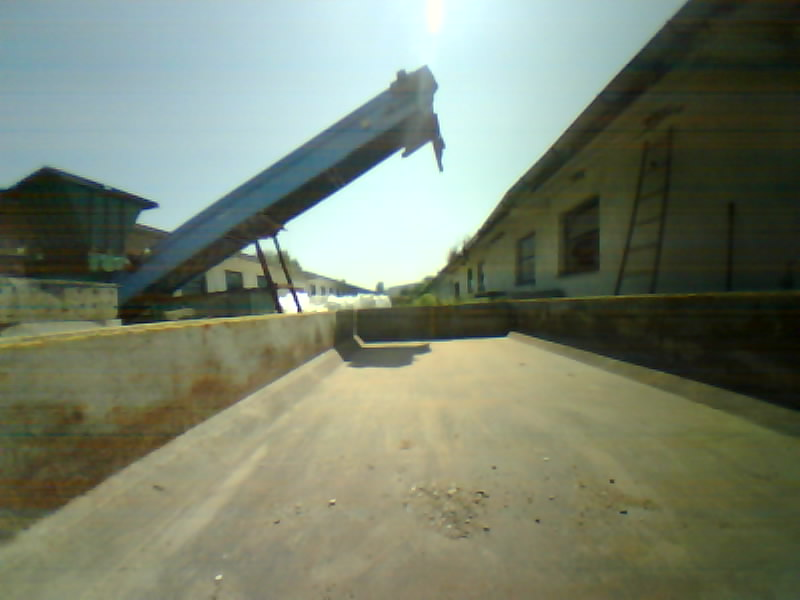
\includegraphics[width=0.7\textwidth]{tex_photos/container_empty.jpg}
    \caption{Example photo taken from the IoT unit camera, showing an empty demolition container.}
    \label{fig:container-empty}
\end{figure}

The data collected by the NB-IoT camera system is visualized and managed through a web dashboard. Figure~\ref{fig:website-dashboard} shows a screenshot of the dashboard, which displays real-time sensor data, fill level, battery status, and location. The dashboard is accessible at \url{https://rm.fsv.cvut.cz/container/5/}.

\begin{figure}[h]
    \centering
    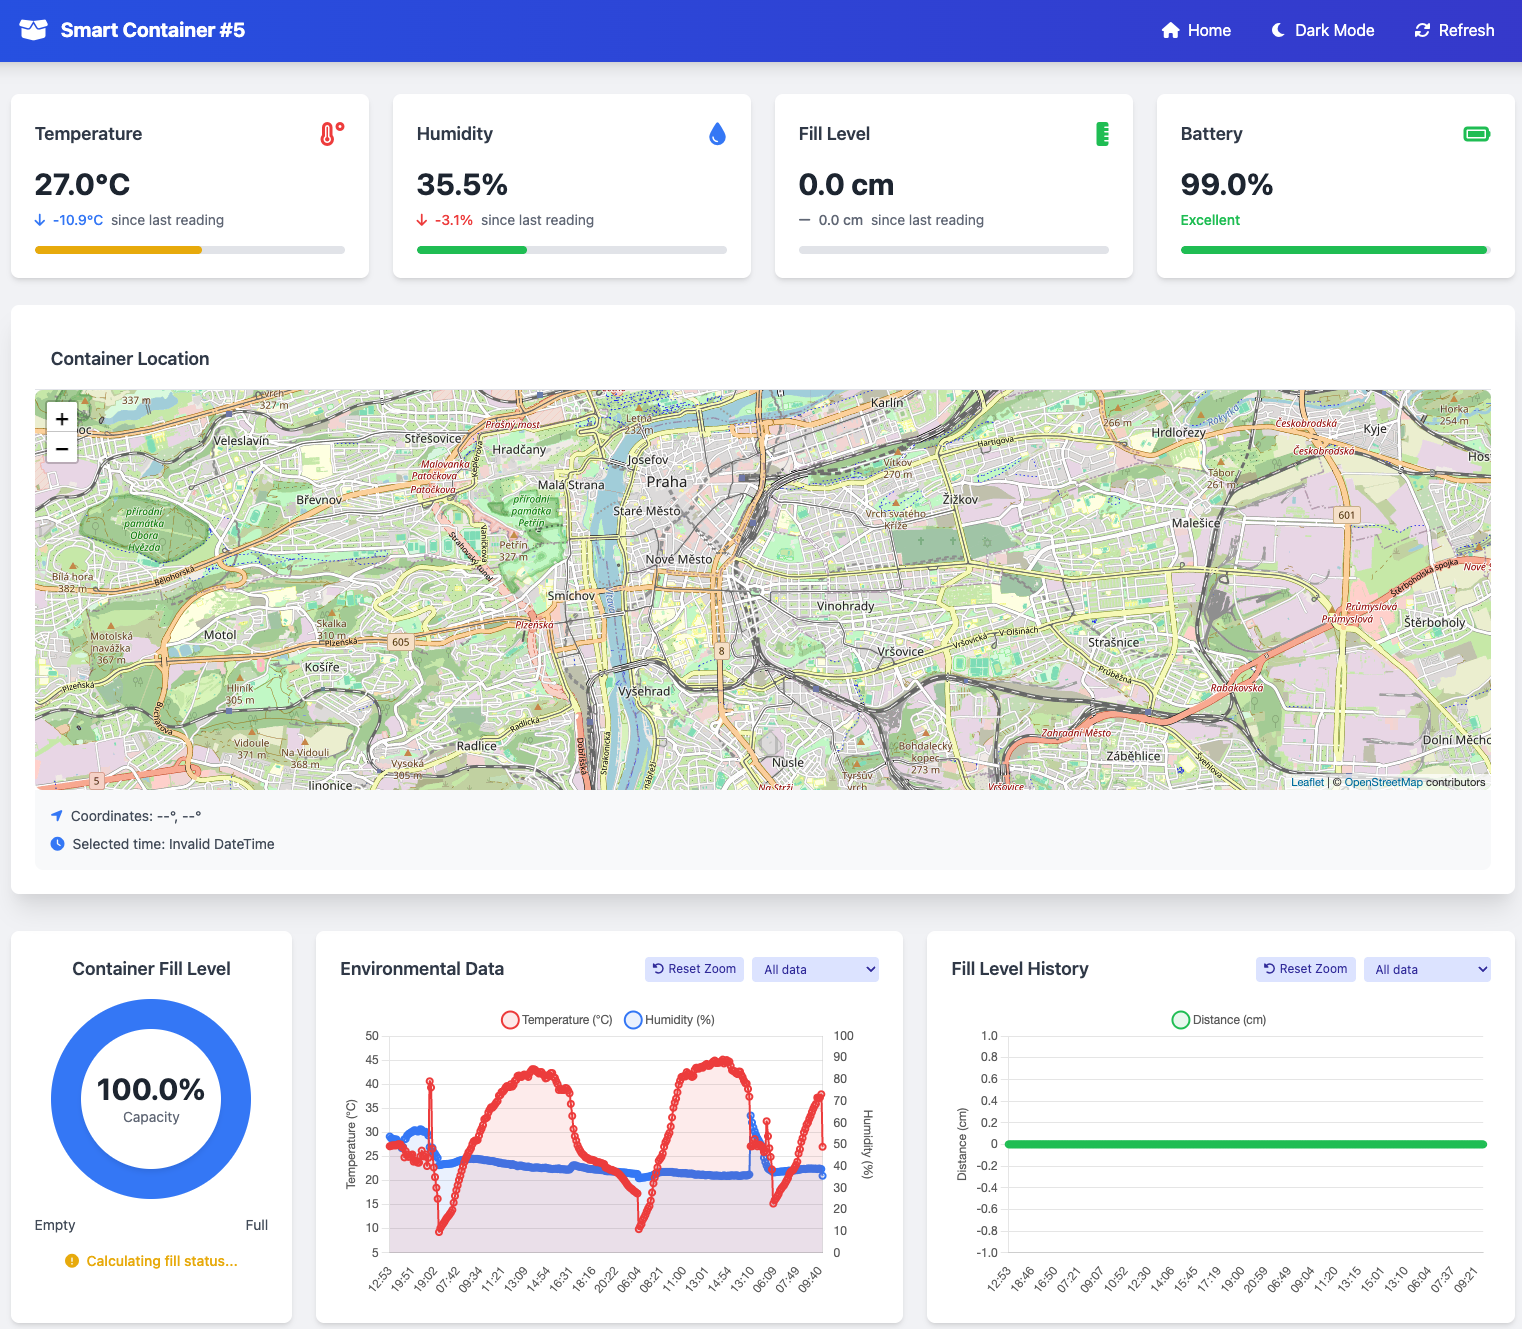
\includegraphics[width=0.95\textwidth]{tex_photos/website_container_5_1}
    \caption{Screenshot of the smart container web dashboard at \url{https://rm.fsv.cvut.cz/container/5/}, showing real-time data and analytics.}
    \label{fig:website-dashboard}
\end{figure}

% After the first dashboard screenshot

\begin{figure}[h]
    \centering
    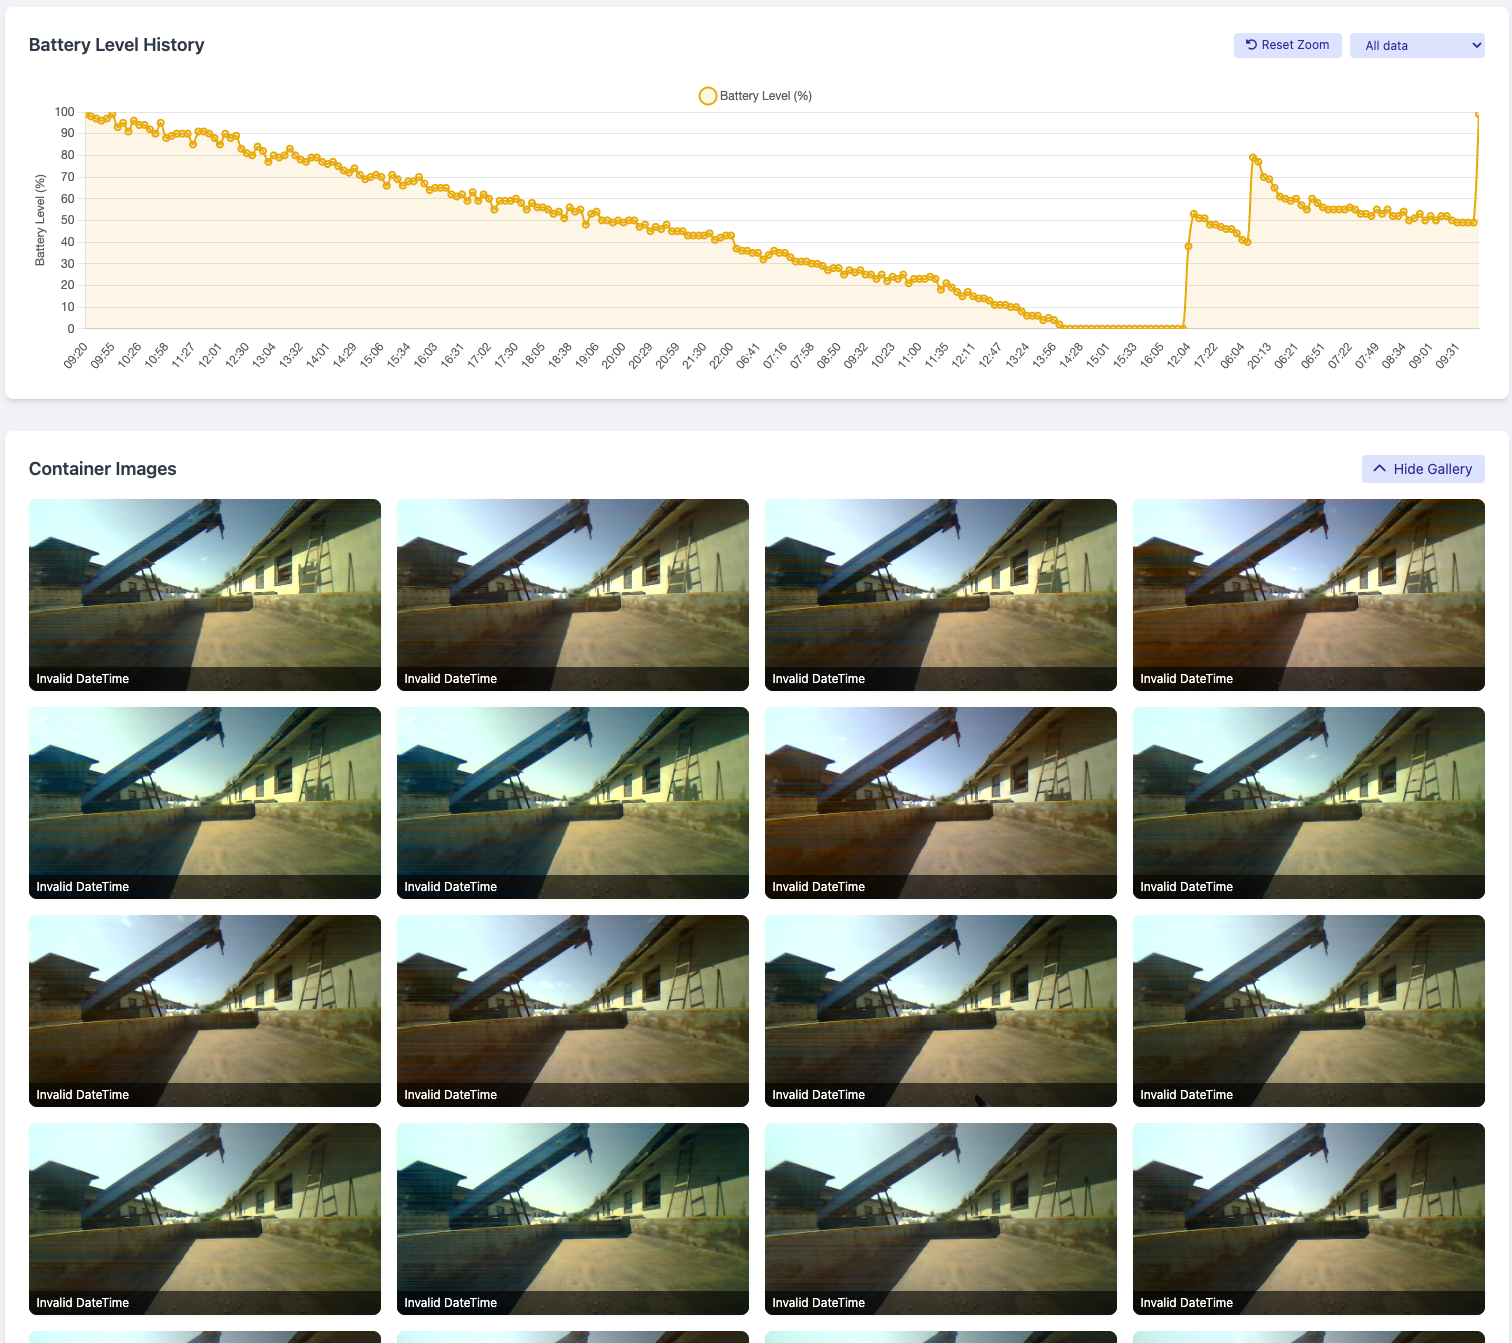
\includegraphics[width=0.95\textwidth]{tex_photos/website_container_5_2}
    \caption{Another view of the smart container web dashboard, showing battery monitoring and photo gallery features.}
    \label{fig:website-dashboard-2}
\end{figure}

\section{Conclusion}

The current ESP32-based NB-IoT camera system demonstrates a robust platform for remote image and sensor data collection in challenging environments. While the present design uses a FireBeetle breakout board for the ESP32-S3, it is important to note that this configuration results in higher power consumption, particularly due to the camera's connection through the breakout. This limitation will be addressed in the next hardware iteration, where the ESP32-S3 will be placed directly on a custom-designed PCB. Prototypes of this new design have already been tested successfully, promising significant improvements in power efficiency and integration.

The primary purpose of the current unit is to collect a diverse dataset of images from the field. These images will be used to develop and train machine learning models for automated image analysis. In future versions, the trained model will be deployed directly on the device, enabling real-time, on-device inference. This approach will drastically reduce the need to transmit large volumes of image data, saving both bandwidth and energy. The device will be able to provide users with actionable information, such as container fill level and material classification, and transmit only images deemed important by the operator—such as those indicating a violation of allowed materials or other critical events.

This evolution will transform the NB-IoT camera system from a data collection tool into an intelligent edge device, capable of delivering timely and relevant insights while maintaining ultra-low power operation. The flexible architecture and ongoing hardware improvements ensure that the system can adapt to new requirements and continue to provide value in a wide range of smart monitoring applications.

\vspace{1cm}
\begin{center}
\textit{For more information, code examples, and real-time data visualization, please visit:}

\href{https://rm.fsv.cvut.cz}{rm.fsv.cvut.cz}\\

% \href{https://www.iot-magic.com}{www.iot-magic.com} // no landing page, just DNS namecheap for the IP
\end{center}

\begin{thebibliography}{9}
\bibitem{esp32}
Espressif Systems, ``ESP32-S3 Series Datasheet,'' 2021.

\bibitem{bc95}
Quectel, ``BC95-G Hardware Design,'' 2020.

\bibitem{ov2640}
OmniVision, ``OV2640 Camera Module Datasheet,'' 2019.

\bibitem{axp313a}
X-Powers, ``AXP313A Power Management IC Datasheet,'' 2020.

\bibitem{gnss}
DFRobot, ``GNSS Module Documentation,'' 2020.
\end{thebibliography}

\appendix

\section*{Appendix: IoT Server Setup Summary (Node-RED, InfluxDB 2.x, Grafana, UDP/TCP)}

The following components were successfully configured and validated on the Google Cloud VM instance:

\begin{itemize}
  \item \textbf{Node-RED} running and listening on custom ports
  \item \textbf{InfluxDB 3 removed}, InfluxDB 2.x installed and initialized with web UI
  \item \textbf{Grafana} installed and connected to InfluxDB 2.x
  \item Custom \textbf{Node-RED flow} parsing UDP payloads into InfluxDB-ready format
  \item Successfully tested \textbf{TCP and UDP connectivity} on ports 8009 and 8094
\end{itemize}

\subsection*{Installed Services}

\subsubsection*{Node-RED}
\begin{itemize}
  \item Installed with \texttt{npm install -g --unsafe-perm node-red}
  \item Run as a persistent service using PM2:
  \begin{lstlisting}[language=bash]
pm2 start $(which node-red) -- -v
pm2 save
pm2 startup
\end{lstlisting}
  \item Configured to accept:
    \begin{itemize}
      \item TCP connections on port \texttt{8009}
      \item UDP messages on port \texttt{8094}
    \end{itemize}
\end{itemize}

\subsubsection*{InfluxDB 2.x}
\begin{itemize}
  \item Removed InfluxDB 3.x
  \item Installed 2.x via:
  \begin{lstlisting}[language=bash]
curl -s https://repos.influxdata.com/influxdata-archive_compat.key | \
  gpg --dearmor | sudo tee /usr/share/keyrings/influxdb-archive-keyring.gpg > /dev/null

echo "deb [signed-by=/usr/share/keyrings/influxdb-archive-keyring.gpg] \
  https://repos.influxdata.com/debian stable main" | \
  sudo tee /etc/apt/sources.list.d/influxdb.list

sudo apt update
sudo apt install influxdb2
\end{lstlisting}
  \item Web UI available at \texttt{http://iot-magic.com:8086}
  \item Created:
    \begin{itemize}
      \item Bucket: \texttt{container}
      \item Organization: \texttt{iot}
      \item Token: \texttt{iot-write-token}
    \end{itemize}
\end{itemize}

\subsubsection*{Grafana}
\begin{itemize}
  \item Installed via:
  \begin{lstlisting}[language=bash]
curl -fsSL https://apt.grafana.com/gpg.key | \
  sudo gpg --dearmor -o /etc/apt/keyrings/grafana.gpg

echo "deb [signed-by=/etc/apt/keyrings/grafana.gpg] \
  https://apt.grafana.com stable main" | \
  sudo tee /etc/apt/sources.list.d/grafana.list

sudo apt update
sudo apt install grafana
sudo systemctl enable grafana-server
sudo systemctl start grafana-server
\end{lstlisting}
  \item Access at \texttt{http://iot-magic.com:3000}
  \item Connected to InfluxDB using token and Flux queries
  \item Implemented:
    \begin{itemize}
      \item State timeline panel for \texttt{wakeUpReasonText}
      \item Geomap panel with \texttt{latitude}, \texttt{longitude}, \texttt{RSSI}
      \item Highlighted latest known device position using \texttt{last()} query
    \end{itemize}
\end{itemize}

\subsection*{UDP Integration and Message Format}

\subsubsection*{UDP Payload Format}
Node-RED receives messages like:
\begin{lstlisting}
sensor temperature=22.5,humidity=65,latitude=50.0875,longitude=14.4213,battery=89
\end{lstlisting}

\subsubsection*{Node-RED Function Logic}
\begin{itemize}
  \item Parses UDP \texttt{msg.payload} (as Buffer)
  \item Splits key=value fields
  \item Creates structured JSON for InfluxDB:
\end{itemize}

\begin{lstlisting}[language=JavaScript]
{
  temperature: 22.5,
  humidity: 65,
  distance: 0,
  latitude: 50.0875,
  longitude: 14.4213,
  container_id: 5,
  image_status: 1,
  battery_status: 89,
  gps_fix_time: 0,
  wake_up_reason: 0
}
\end{lstlisting}

\subsection*{Connectivity Tests}

\subsubsection*{Local Port Checks}
\begin{lstlisting}[language=bash]
sudo apt install lsof
sudo lsof -i -n -P | grep -E '8009|8094'
\end{lstlisting}

\subsubsection*{Local UDP/TCP Sending}
\begin{lstlisting}[language=bash]
echo "hello tcp" | nc 127.0.0.1 8009
echo "hello udp" | nc -u 127.0.0.1 8094
\end{lstlisting}

\subsubsection*{Remote UDP Sending Example}
\begin{lstlisting}[language=bash]
echo "sensor temperature=22.5,humidity=65,latitude=50.0875,longitude=14.4213,battery=89" \
  | nc -u <your-vm-ip> 8094
\end{lstlisting}

\subsection*{ESP32 Wake-Up Reason Codes}
Used for mapping \texttt{wakeUpReason} integers:

\begin{table}[h]
\centering
\begin{tabular}{|c|l|}
\hline
Code & Meaning \\
\hline
0 & ESP\_SLEEP\_WAKEUP\_UNDEFINED \\
1 & ESP\_SLEEP\_WAKEUP\_EXT0 (RTC\_IO) \\
2 & ESP\_SLEEP\_WAKEUP\_EXT1 (RTC\_CNTL) \\
3 & ESP\_SLEEP\_WAKEUP\_TIMER \\
4 & ESP\_SLEEP\_WAKEUP\_TOUCHPAD \\
5 & ESP\_SLEEP\_WAKEUP\_ULP \\
6 & ESP\_SLEEP\_WAKEUP\_GPIO \\
7 & ESP\_SLEEP\_WAKEUP\_UART \\
8 & ESP\_SLEEP\_WAKEUP\_WIFI \\
9 & ESP\_SLEEP\_WAKEUP\_COCPU \\
10 & ESP\_SLEEP\_WAKEUP\_COCPU\_TRAP \\
11 & ESP\_SLEEP\_WAKEUP\_BT \\
\hline
\end{tabular}
\caption{ESP32 wake-up reason codes}
\end{table}

\end{document} 